\chapter{Proposed Solution}
\label{cap:method}

\intro{In this chapter, the proposed solution is presented. The chapter is divided into two sections: architecture, and implementation. The architecture section describes how a cloud-agnostic architecture capable of collecting, processing, and storing data from IoT devices and archived data can be designed. The implementation section present a test implementation of the proposed solution that demonstrate the feasibility of the architecture and its cloud-agnostic nature.}\\


\section{Architecture}
\label{sec:architecture}
\begin{figure}[htbp]
    \centering
    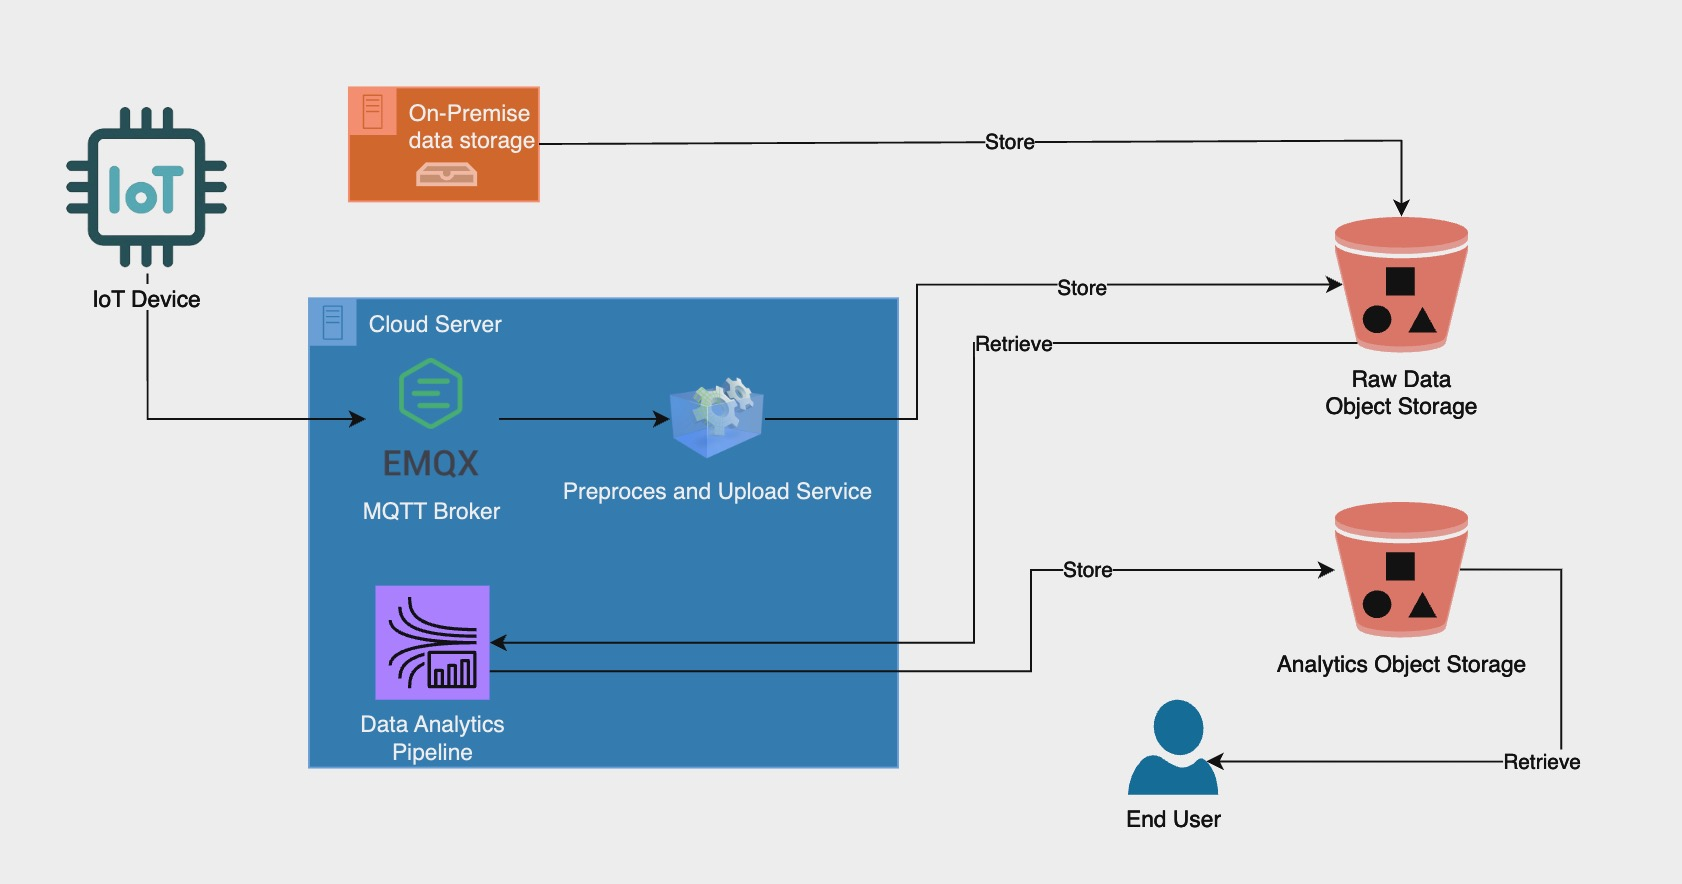
\includegraphics[width=1\textwidth]{architecture.png}
    \caption{Architecture of the proposed solution}
    \label{fig:architecture}
\end{figure}
The proposed solution's architecture consists of a composition of loosely coupled microservices\footnote{Loosely coupling is an approach in programming that aims to limit as much as possible the dependencies between different components}\footnote{Microservices is an architectural style that consists in dividing a large application in many smaller parts that are able to work independently from one another} that work together to collect, process, and store data. The architecture is divided into three layers: the data collection layer, the data storage layer and the data analysis layer. Each layer plays a specific role in the overall system, ensuring scalability, flexibility, and resilience. A schema representing the architecture is shown in figure \ref{fig:architecture}.

\subsection{Data Collection Layer}

The data collection layer is responsible for gathering data from IoT devices and archived on-premise data. 

\subsubsection{Data Collection from IoT Devices}
In our setup, numerous IoT devices can send data to the cloud via MQTT to a specific MQTT broker. The broker is hosted on a cloud server and is accessible to all IoT devices connected to the network. The broker is configured to use a specific topic\footnote{A topic, when talking about MQTT protocol, is defined by a string. Each device when publishing messages will use a specific topic. All the subscribers of that specific topic are able to see the messages.} for each device, ensuring that messages are delivered to the correct destination. Each device is configured to publish data on a specific topic, which is managed by a cloud-based broker. The data containing a timestamp and key-value pairs representing sensor readings is sent in JSON\footnote{JSON is a popular data exchange format based on JavaScript programming language. It's widely used in API development and IoT fields. It usually consists of key-value pairs. Each value can be an atomic value, an object or even an array of objects.} format. Once the data reaches the broker, it is preprocessed before storage. This preprocessing step involves parsing the JSON data, extracting the timestamp and sensor values, and converting the data to CSV format\footnote{CSV (Comma Separated Values) is a lightweight format for exchanging data. It usually consists of an header and a number of rows where each column is separated by the colon character and each row by the newline character.}. CSV was chosen for its simplicity, broad compatibility with data processing tools, and because it's less verbose than JSON. Finally, the preprocessed data is stored in object storage, where it can be accessed by the data processing pipeline.


\subsubsection{Data Collection from Archived Data}
To collect data from archived sources, files from on-premises systems are uploaded to the cloud using a straightforward script that leverages cloud's API. Since these files are already in CSV format no preprocessing is needed, so they are directly uploaded to object storage, making them readily accessible for the data processing pipeline. These files hold historical data that has been gathered over time across different scenarios.

\subsection{Data Storage Layer}

The data storage layer is designed to store raw and analyzed CSV data. It ensures that row data are available for the processing pipeline and that analyzed data are stored for future use. Raw data and analysis outputs are saved in different buckets\footnote{In Object Storage, a bucket is a container able to store object within a specific namespace.} to ensure a less complicated data management pipeline.
This layer can leverage on any Object Storage service offered by any provider since all of them are cost effective, scalable and redundat. 

\subsection{Data Analysis Layer}

The data analysis layer is dedicated to examining the collected data and generating meaningful insights. This layer comprises multiple services that retrieve preprocessed data from object storage to carry out various analytical tasks. The data is first downloaded from the object storage to a local storage leveraging the object storage APIs. This needs to be done since Object Storage services do not allow to access the content of the files directly.

Once the data is retrieved one or more analytics services run to analyze the data. These services can leverage simple statistical assessments as well as more advanced machine learning and deep learning techniques.
The analysis process extracts valuable insights that can be showed to the users of a certain application to enhance their experience. 
The analyzed data are then saved in the object storage again, but in a different bucket making them accessible for future use by other services or users.
There is the possibility to start the analysis automatically when new data is uploaded to the object storage, or to trigger it manually for example implementing a set of APIs\footnote{An API (Application Programming Interface) is a piece of software that aims to facilitate the information exchange between a server and some other software.} that can be called by the user. This is an implementation choice that depends on the specific requirements of the project and that cannot be decided at a general architectural level.

\subsection{Cloud Server (IaaS) vs. SaaS Solutions}

The usage of a cloud server to host both the MQTT broker and the data analytics pipeline offers many advantages with respect to a SaaS solution.
A SaaS architectures can be convenient with respect to a IaaS one when talking about management and responsibilities. On the other hand, an IaaS based architecture allows for more flexibility and control of the underlying infrastructure. This can be especially useful in case that custom configurations and dependencies are needed for the data analytics pipeline.
A cloud server allows for better cost management with the only downside being the responsibility of managing the operating system and applying security patches. In contrast, SaaS solutions, are generally easier to set up and maintain but can also have higher costs over time due to higher subscription fees.
The cloud server approach is also inherently cloud-agnostic since every provider offers an IaaS service. This aspect ensures that users can select the cloud provider that best fits with their requirements without needing to change the architectural design of the solutions. With this solution, the MQTT broker and the data analytics pipeline are hosted on the same server but they function independently so the principles of microservices architectures are respected.
In summary, this architecture is robust, scalable, and flexible. Its cloud-agnostic nature allows for an easy implementation with any provider in the market. Furthermore, the cost-effective design can be particularly important for long-term projects. This approach not only meets the immediate operational needs but also positions organizations to adapt and evolve as their requirements change over time.

\subsection{Why the proposed architecture is cloud-agnostic}
The proposed architecture is designed to work with any cloud provider. Considering the cloud services described in \ref{cloud}, the architecture can be implemented using any of providers since each of them offers some Object Storage and some computing services. The data storage layer in the design uses an Object Storage service to store raw and preprocessed data. This layer can be implemented using any cloud provider's Object Storage service, as all providers offer similar services. The data analysis layer uses a cloud server to run the data processing pipeline. This layer can be implemented using any cloud provider's IaaS service and with every operative system, as all providers offer similar services. The data collection layer instead uses a MQTT broker to collect data from IoT devices. This layer can be implemented using any cloud provider's MQTT broker service, as well as on a computing service where a MQTT broker can be installed. Considered the fact that the same base architecture can be implemented using any cloud provider, the proposed solution can be considered cloud-agnostic.
\section{Test Implementation}

In this section, the base implementation of the proposed solution is presented. The implementation is divided into two main components: the data collection layer, the data storage layer and the data analysis layer. The data collection component is responsible for collecting data from IoT devices and archived data, while the data analysis component is responsible for processing and analyzing the collected data. In this implementation to test the cloud agnostic nature of the architecture, each layer has been implemented using both Azure and Aruba. The implementation is based on the architecture described in \ref{sec:architecture} and aims to demonstrate the feasibility of the proposed solution. 

\subsection{Data Collection layer}

The data collection component is responsible for collecting data from IoT devices and archived data. This component consists of three main parts: the MQTT broker, the preprocessing pipeline and the data upload script.

\subsubsection{MQTT Broker}
MQTT broker is a lightweight messaging broker that implements the MQTT protocol. The broker is responsible for receiving messages from IoT devices and forwarding them to subscribers.  
The broker that we have chosen for the test implementation \href{https://www.emqx.io/}{EMQX}, whose pros and cons have been discussed in \ref{emqx}.
Once the broker was been installed and configured in the cloud server, it was tested by connecting some simulated IoT devices which was then sending messages to the broker. The messages were successfully received by the broker and forwarded to the subscriber, demonstrating the broker's functionality.
The IoT devices used in the test were simulated using the \href{https://mqttx.app/}{MQTTX} client, analyzed in \ref{mqttx} . This MQTT client allows users to simulate IoT devices and publish messages to an MQTT broker. The simulated devices were configured to publish JSON messages to the broker using a specific topic, with each of the messages containing a timestamp and a set of key-value pairs representing the data.

\subsubsection{Preprocessing pipeline}
The preprocessing pipeline is responsible for parsing the JSON data received from the MQTT broker, extracting the timestamp and key-value pairs, and converting the data to CSV format. The pipeline is implemented as a Python script that thanks to \href{https://pypi.org/project/paho-mqtt/}{paho-mqtt}\footcite{site:paho-mqtt}, an MQTT client library for Python, subscribes to the MQTT broker, receives messages, and preprocesses the data. Once the data is received, it is parsed, and the timestamp and key-value pairs are extracted. The data is then converted to CSV format and stored in object storage. The preprocessing pipeline ensures that the data is in a suitable format for further analysis and processing. The script was tested by connecting it to the MQTT broker and receiving messages from the simulated IoT devices. The messages were successfully parsed, and the data was converted to CSV format, demonstrating the pipeline's functionality.

\subsubsection{Data Upload Script}
The data upload script is responsible for uploading archived data from on-premises to the cloud. The script is implemented as a Python script that uses the cloud provider's API to upload files to object storage. The script reads the files from a local directory, uploads them to object storage, and makes them accessible to the data processing pipeline. In this scenario the files are already stored in CSV format, making them suitable for direct upload to object storage. The script was tested by uploading several sample files to object storage and verifying that the files were successfully uploaded to the right directory and accessible to the data processing pipeline. 

\subsection{Data Storage Layer}
The data storage layer is responsible for storing raw and analyzed data. This layer ensures that raw data is available for the processing pipeline and that analyzed data is stored for future use. The data storage layer consists simply of an object storage service. Each cloud provider analyzed in \ref{cloud} offers an object storage service with a set of APIs that allow users to store and retrieve data, since the API can vary from provider to provider, all the scripts interacting with the storage itself have been developed to be able to work with both Azure and Aruba. The data storage layer was tested by uploading raw and analyzed data to object storage and verifying that the data was successfully stored and accessible to the data processing pipeline.
\begin{figure}[htbp]
    \centering
    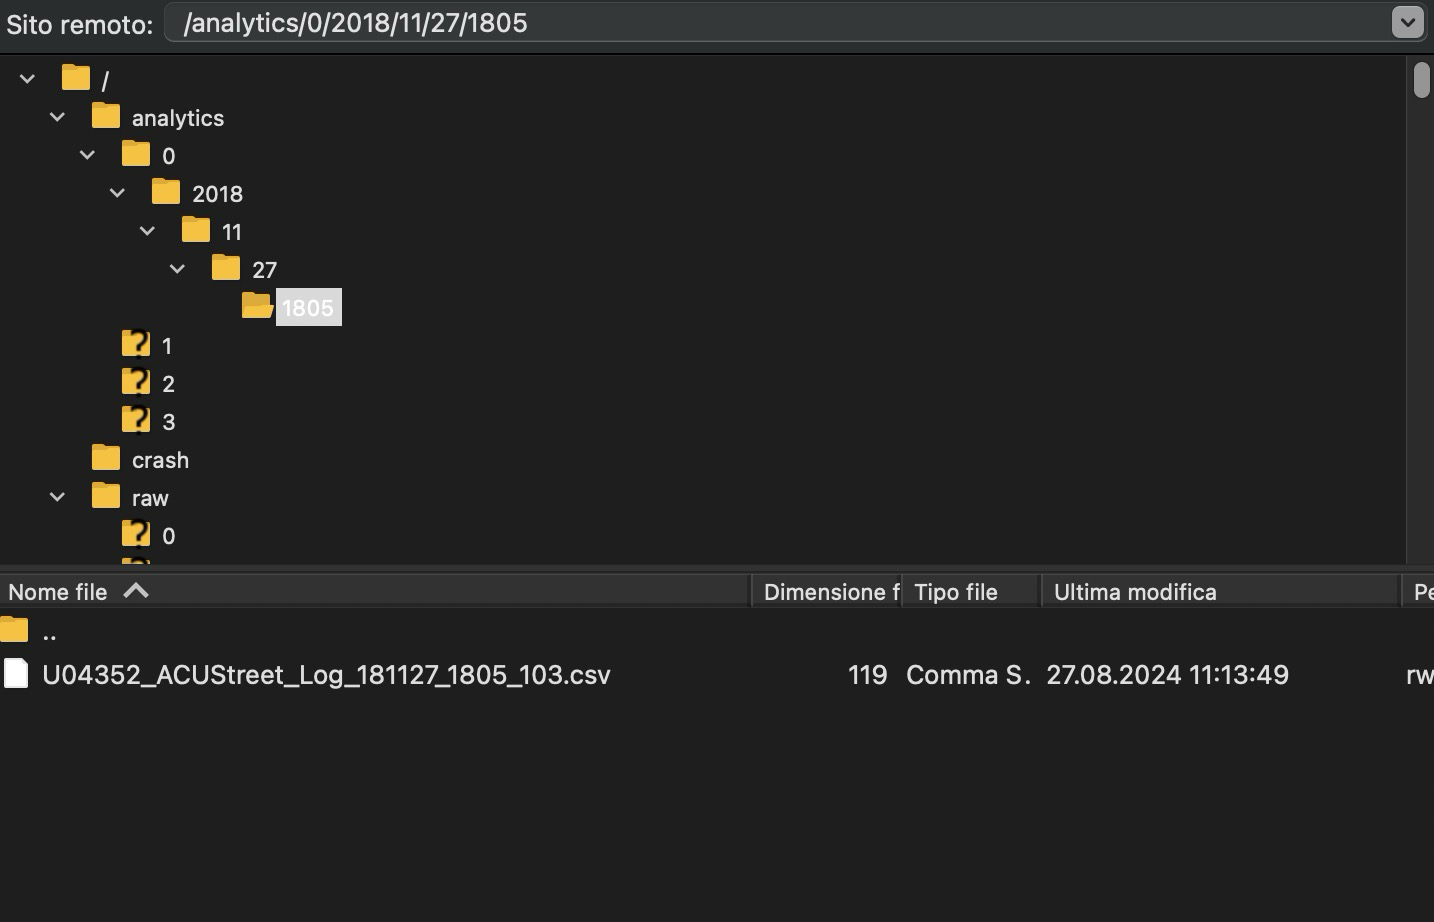
\includegraphics[width=1\textwidth]{data_storage.png}
    \caption{Example of an analytics CSV file stored in object storage}
    \label{fig:storage}
\end{figure}


\subsection{Data Analysis Component}
The data analysis component is responsible for processing and analyzing the collected data. This component can consist of one or more data analytics scripts based on the requirements of the project. Each of the scripts needs to retrieve the correct data from the object storage, perform the required analysis, and store the results in a separate object storage bucket. In the case more than one file needs to be retrieved from storage, the scripts need to manage the data retrieval and processing sequentially to optimize performance and resource usage. The scripts can be implemented in any programming language that supports the required data processing and analysis tasks. The choice of language depends on the specific requirements of the project and the availability of libraries and tools for data processing and analysis.
This component was tested by implementing  a simple data analysis script that retrieves the preprocessed data from object storage, calculates simple statistics, and stores the results in a separate object storage bucket. The script was implemented in Python using various Python libraries such as Pandas and NumPy for data manipulation and analysis. The script was tested by retrieving the preprocessed data from object storage, calculating the statistics, and storing the results in a separate object storage bucket. The results were successfully stored, demonstrating the functionality of the data analysis component.
Once the analytics are uploaded they can be accessed via a web interface or a REST API, depending on the requirements of the project. The results can be visualized using various data visualization tools such as \href{https://matplotlib.org/}{Matplotlib}\footcite{site:matplot}, \href{https://plotly.com/}{Plotly}\footcite{site:plotly}, or \href{https://grafana.com/}{Grafana}\footcite{site:grafana}, providing insights into the underlying patterns and trends in the collected data.
